% Encoding: utf-8
% Project documentation.
\documentclass[a4paper,10pt]{article}

% Packages
\usepackage[utf8]{inputenc}
\usepackage{czech}
\usepackage{url}
\usepackage{graphicx}
% \usepackage{unicode-math}

% Omicron fake (because I am not using proper pdflatex compiler)
\newcommand{\Omicron}{O}

\title{Paralelní a distribuované algoritmy \\Projekt č. 3 \-- Implementace Mesh Multiplication}
\author{Daniel Dušek, xdusek21@stud.fit.vutbr.cz}

% Some pretty neat values, probably figured out by Petr Zemek (https://github.com/s3rvac)
\setlength{\hoffset}{-1.5cm}
\setlength{\voffset}{-1.5cm}
\setlength{\textheight}{23.0cm}
\setlength{\textwidth}{15.2cm}

\begin{document}

    \maketitle

	\section{Rozbor a analýza algoritmu}
	\par Mesh Multiplication algoritmus je navržen pro výpočet násobení matic na architektuře procesorů zapojených do mřížky. Mřížka počítajících procesorů vždy bude mít stejný počet sloupců a řádků jako výsledná matice získaná násobením matic na vstupu. Pro vstupní matice A ($m*n$) a B ($n*k$) je tedy vytvořena mřížka $m*k$ procesorů. Jednotlivé řádky, resp. sloupce této mřížky jsou číslovány od 1 do $m$, resp. od 1 do $k$. Na procesory umístěné v~prvním řádku, popřípadě prvním sloupci, jsou přiváděny odpovídající hodnoty ze vstupních matic a to tak, že pro násobení matic $A*B$ dostávají procesory umístěné v~prvním sloupci postupně hodnoty řádků matice $A$ a procesory umístěné v~prvním řádku dostávají postupně hodnoty sloupců matice $B$.

	\par Každý procesor získá vždy dvě hodnoty \-- hodnotu z matice $A$ a hodnotu z matice $B$ \-- buď od~svého souseda vlevo a nad sebou, nebo, nemá-li souseda, čte hodnoty z paměti tak, jak je popsáno výše. Tyto dvě hodnoty vždy spolu vynásobí a přičte je k hodnotě svého vnitřního registru C (na~začátku nastaven na 0, na konci algoritmu obsahuje číslo v matici na pozici procesoru).

	\hspace{0.2cm}

	\textbf{Princip výpočtu a předávání hodnot v algoritmu Mesh Multiplication mezi procesory (při násobení výše zmíněných matic $A*B$)}

	\begin{enumerate}
		\item Procesor $P_{i,j}$ obdrží hodnoty dvou vstupů $a$ a $b$.
		\item Procesor hodnoty vstupů $a$ a $b$ vynásobí.
		\item Přičte získanou hodnotu k hodnotě svého registru $C_{i,j}$.
		\item Pokud není pravda, že $j = k$, pak pošle hodnotu $a$ procesoru $P_{i,j+1}$.
		\item Pokud není pravda, že $i = m$, pak pošle hodnotu $b$ procesoru $P_{i+1,j}$.
	\end{enumerate}

	\par Prvkům $a_{m1}$ a $b_{1k}$ trvá $m+k+n-2$ kroků než dojdou do procesoru $P(m,k)$. Procesor $P(m,k)$ je poslední a jeho výpočtem celý algoritmus končí. Za předpokladu, že $m \leq n$ a $k\leq n$ běží algoritmus v čase $t\left(n\right) = \Omicron\left(n\right)$. Dále odvozujeme, že $p\left(n\right) = \Omicron\left(n^2\right)$ a tedy i $c\left(n\right) = \Omicron\left(n^3\right)$ což odpovídá ceně provedení sekvenčního algoritmu pro násobení matic a tedy, algoritmus není optimální.

	
	\section{Implementace}
	\label{sec:implementace}
    	\par Jako implementační jazyk byl zvolen jazyk C++ s využitím knihovny Open MPI. 

    	\par Kód programu je rozdělen do dvou význačných větví: větev pro procesor, který je umístěn na~souřadnicích $[0,0]$ a je považován za \uv{řídící} a větev pro všechny ostatní procesory. V každé větvi je pak samostatný cyklus, který se provede v závilosti na počtu řádků vstupní matice $A$ \-- tedy pro matici $m*n$ se provede m-krát. Zvolený řídící proces provádí to, že v každé iteraci cyklu čte vstupní hodnoty z paměti, ve které jsou matice uloženy (mapovány na 1-D vector). Pro přístup ke správným hodnotám využívá napsanou přístupovou funkci. Dále jsou ve větvi řídícího procesu ošetřené hraniční případy, kdy je například mřížka tvořena pouze řídícím procesorem, řídící procesor nemá souseda v pravo, nebo pod sebou. 

    	\par Ve větvi pro ostatní procesory pak hraje roli, zda se procesor vyskytuje uvnitř mřížky, nebo na~jejím okraji. V případě, že se vyskytuje na jejím horním resp. levém okraji, čte si procesor hodnotu $b$ resp. $a$ z v paměti uložených matic, $B$ a $A$, na druhou při první iteraci čeká pomocí blokující funkce \texttt{MPI\_Recv()}. Po provedení očekávaného kroku algoritmu pak procesor zasílá načtené hodnoty svému pravému a spodnímu sousedovi \-- avšak jen pouze v případě, že zasílající procesor se nevyskytuje na dolním, resp. pravém okraji (případ, kdy mu alespoň jeden ze sousedů chybí). Řadový procesor vyskytující se uvnitř mřížky zahajuje svůj cyklus čekáním výše zmíněnou funkcí na obě hodnoty od svých sousedů.

    	\par Po konci výpočtu násobení matice pak následuje vypsání vypočtených hodnot na vstup. To je realizováno pomocí volání \texttt{MPI\_Send()} pro zaslání obsahu registru C všemi neřídícími procesy a~odchycením této zprávy řídícím procesorem funkcí \texttt{MPI\_Recv()} volanou v cyklu. Řídící procesor pak vypíše rozměry výsledné matice a následně vypíše i prvky této matice. Před samotným vypsáním je pro jistotu využito funkcionality \texttt{MPI\_Barrier()} čekající na globální komunikační skupinu, aby bylo zamezeno tomu, že se řídící procesor pokusí vykonávat svou závěrečnou větev dříve než ostatní procesory skončily práci. 

	\section{Měření a experimenty}
	\label{sec:mereni}

		\par Algoritmus byl testován na celkově 25 maticích, kde počet a rozložení jejich prvků na řádcích a~sloupcích bylo sestavováno tak, aby počet výsledných procesorů potřebných k výpočtu byl roven právě číslu od 1 do 25 (u prvočísel jako jsou 17 či 19 byly využity vektory). Matice byly sestavovány tak, aby výsledná matice po násobení byla co nejblíže čtvercové matici. Limit na 25 procesorů byl vybrán s ohledem na možnost testování na školním serveru \textit{Merlin}. Cílem měření bylo změřit \texttt{reálnou} časovou náročnost algoritmu v závislosti na velikosti a typu vstupních dat. Program byl během měření spuštěn 30-krát pro každou vstupní matici a výsledný čas byl zprůměrován. Z výsledného průměru nebyly tentokrát odstraňovány hodnoty, které řádově nepatřily mezi ostatní, aby byl zachován vliv prostředí. 

		\par Experimenty byly provedeny na školním testovacím server \textit{Merlin} a výsledný časový trend byl takřka shodný s trendem naměřeným na autorově stanici. Časově se hodnoty ovšem lišily \-- na školním serveru byly řádově nižší (toto si autor vysvětluje jako rozdíl v HW konfiguraci), a obsahovaly více hodnot diametrálně mimo běžné řády hodnot.

		\par Pro měření doby běhu skriptu bylo využito funkce \texttt{MPI\_Wtime()} volané na dvou vhodných místech v~kódu \-- a sice po initiálním načtení hodnot a zařízením jejich přístupnosti odpovídajícím procesorům, a po konci násobícího algoritmu, kdy poslední procesor provedl finální výpočet. Umístění měřícího kódu do těchto míst je dostatečné a oprávněné, neb moment, kdy poslední procesor vynásobí poslední příchozí hodnoty a přičte je k hodnotě svého registru C, algoritmus Mesh Multiplication doběhl. Dvě získané hodnoty od sebe potom byly odečteny a tím byla získána opravdová doba běhu algoritmu. 
    	
    	\par V grafu~1 je vyobrazena naměřená závislost časové náročnosti na velikosti vstupních dat a počtu pracujích procesorů.  

			\begin{figure}[th]
			\centering
			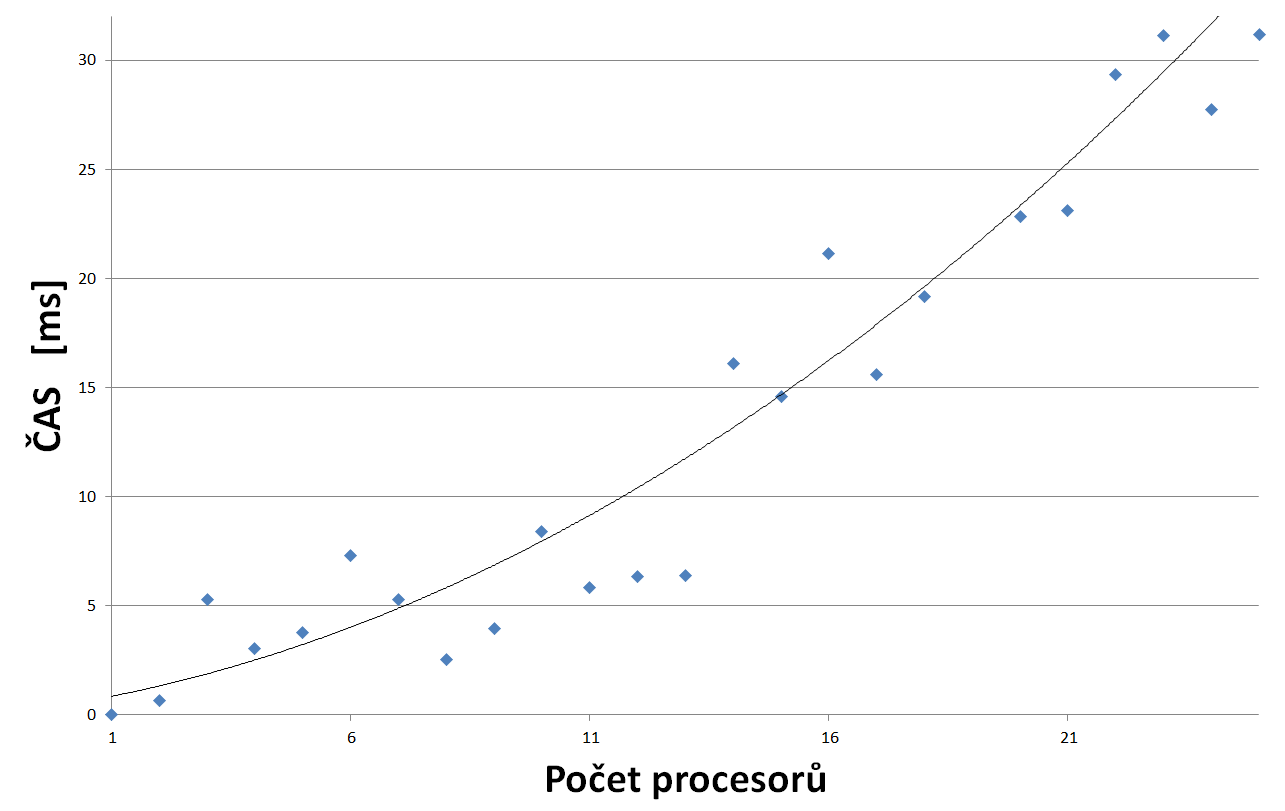
\includegraphics[width=0.85\textwidth]{graferino.PNG}
			\label{fig:graph}
			\caption{Graf závislosti časové náročnosti na velikosti vstupních dat (a počtu pracujících procesorů)}
			\end{figure}	


	\section{Komunikační protokol procesů}
	\label{sec:comprot}
    	\par Meziprocesorová komunikace je simulována pomocí funkcí poskytovaných MPI knihovnou \texttt{MPI\_Recv()} a \texttt{MPI\_Send()}. Knihovna MPI navíc poskytuje další užitečné funkce jako je či \texttt{MPI\_Gather()} s~\texttt{MPI\_Scatter()}, které by mohly být využity při dalších možných optimalizacích implementovaného algoritmu (popsáno níže). Sekvenční diagram meziprocesové komunikace je zachycen na obrázku~2.  %TODO FIX THIS REFERENCE

		\begin{figure}[h!]
    	\centering
    	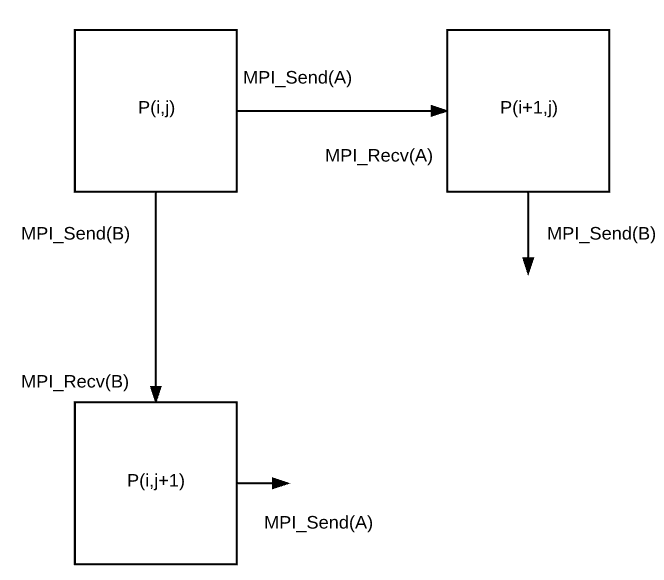
\includegraphics[width=0.75\textwidth]{sequentino.PNG}
    	\label{fig:sequence-diagram}
    	\caption{Sekvenční diagram meziprocesorové komunikace.}
    	\end{figure}

	\section{Závěr}
	\label{sec:terminus}
	\par Experimentálně bylo naměřeno, že časová složitost je polynomická druhého řádu, což ovšem úplně nekoresponduje s tím, co o algoritmu v teoretické rovině víme. Jako hlavní problém zde autor vidí to, že reálně algoritmus není spouštěn na tolika procesorech, na kolika by měl běžet, reálně jsou spouštěny procesy mezi kterými dochází k přepínání kontextů a celkově zde existuje více nadměrné režie, která by u opravdové víceprocesorové architektury takto neovlivňovala výsledky.

\end{document}